    \section{基于深度学习}
    
    \subsection{DehazeNet}
    \begin{frame}
    \frametitle{基于深度学习的去雾算法}
    根据深度学习模型的输出是否为去雾后的清晰图像,可以将基于深度学习的去雾算法分为两类:
    \begin{itemize}
    \item 第一类算法首先通过建立深度学习模型来估计大气散射模型中的未知参数—透射率图,再基于先验理论估计大气光照值,最后根据大气散射模型变形公式恢复对应的无雾图像,即基于非端到端的网络模型实现图像去雾
    \item 第二类算法直接建立深度学习模型恢复无雾图像,即基于端到端的网络
    模型实现图像去雾
    \end{itemize}
    \end{frame}

    \begin{frame}
      \frametitle{DehazeNet}
      \begin{figure}[h]
        \centering
        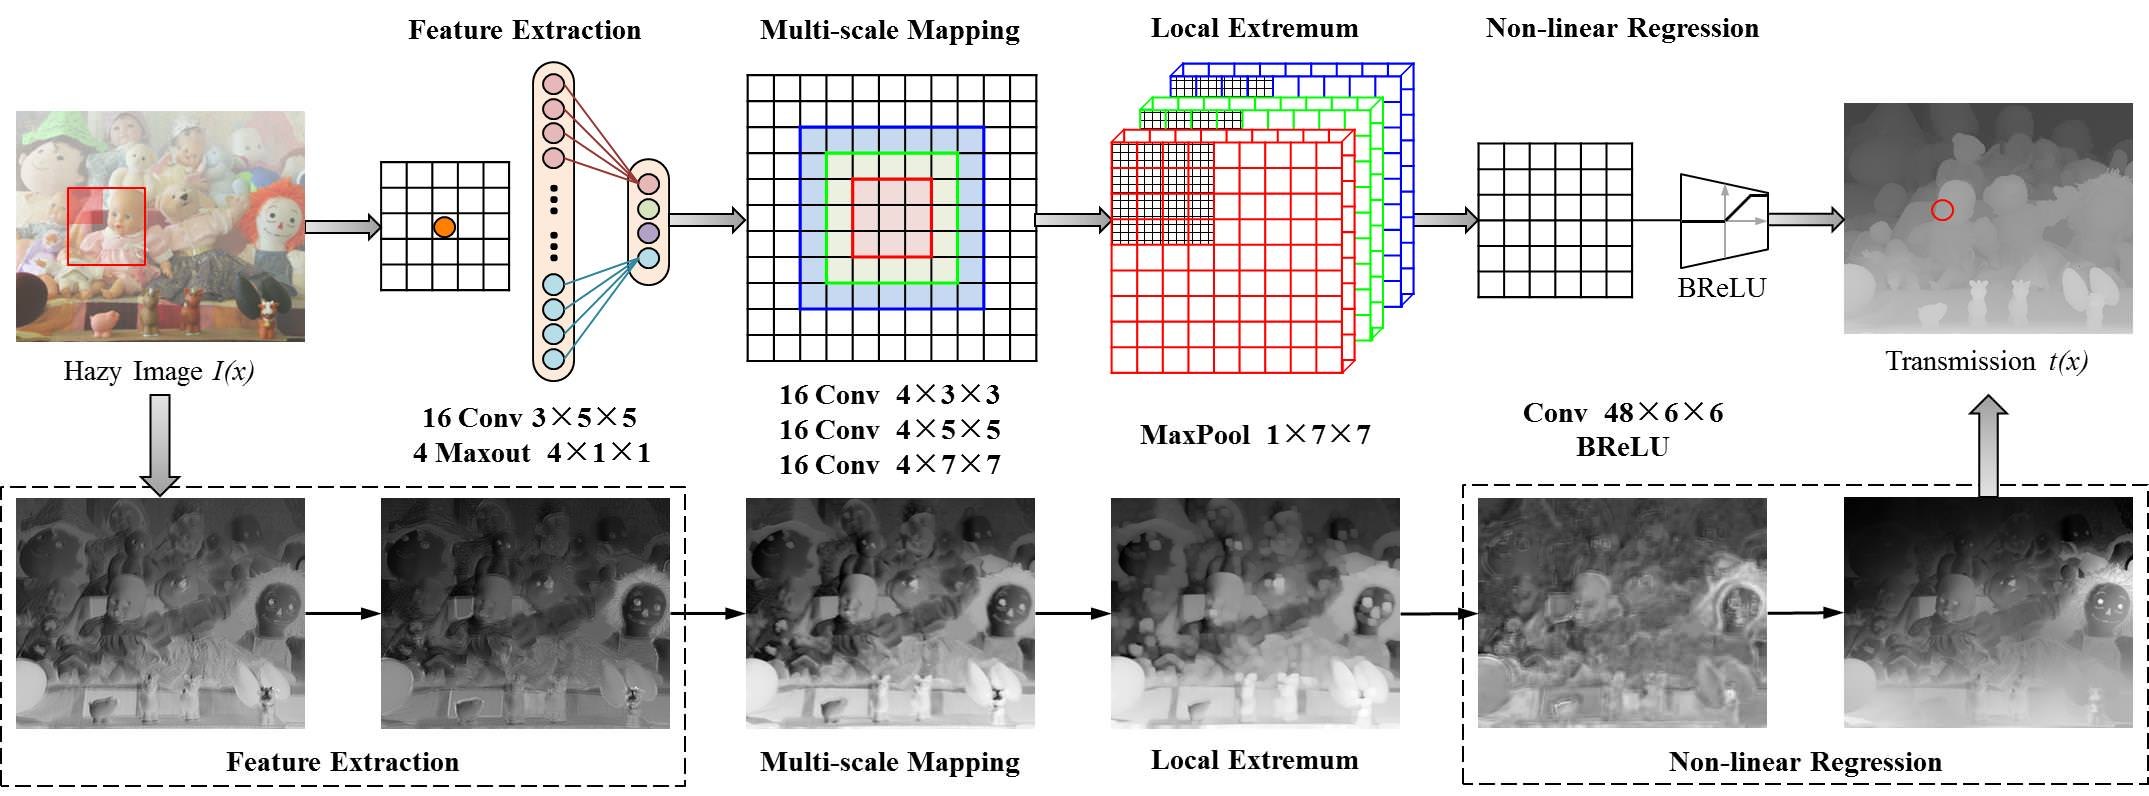
\includegraphics[width=\linewidth]{figures/pic10.png}
        \caption{DehazeNet结构示意图}
      \end{figure}
      \end{frame}

    \begin{frame}
      \frametitle{DehazeNet}
      \begin{figure}[h]
        \centering
        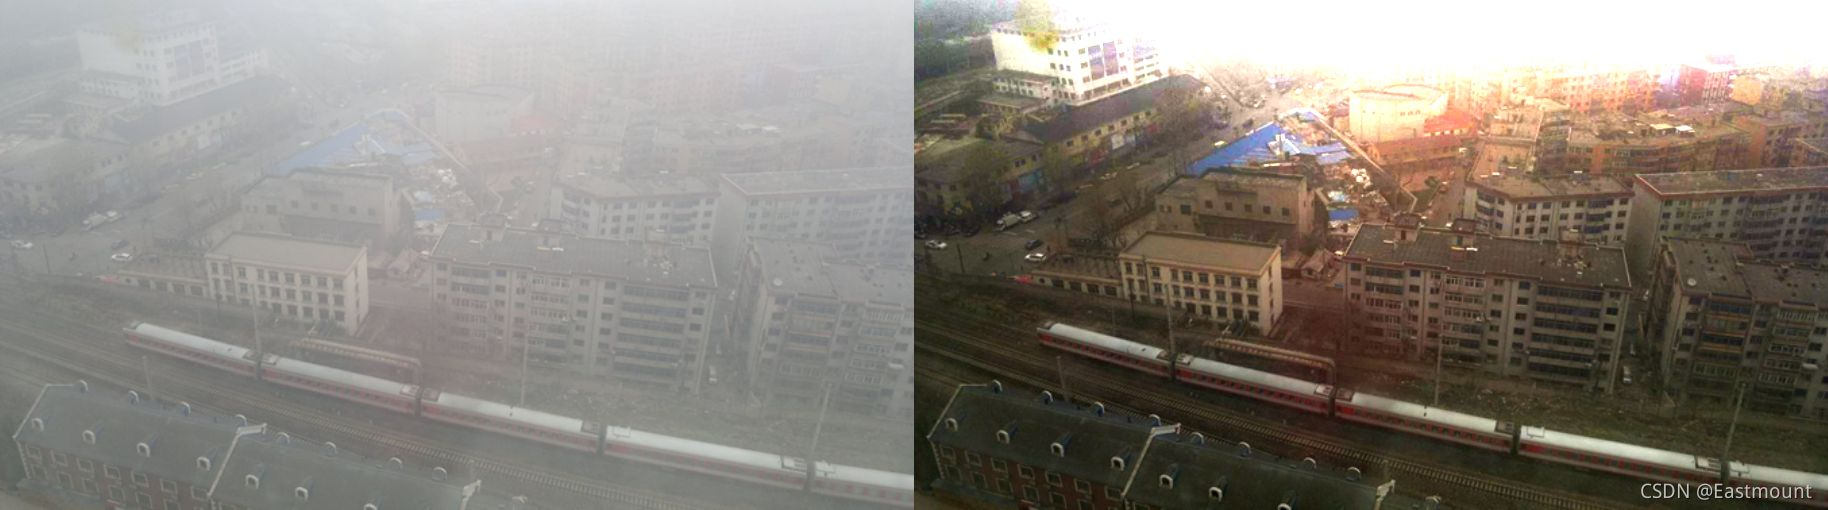
\includegraphics[width=\linewidth]{figures/pic12.jpg}
        \caption{DehazeNet去雾效果图}
      \end{figure}
    \end{frame}
  

    \subsection{AOD-Net}
    \begin{frame}
    \frametitle{AOD-Net}
    \begin{figure}[h]
      \centering
      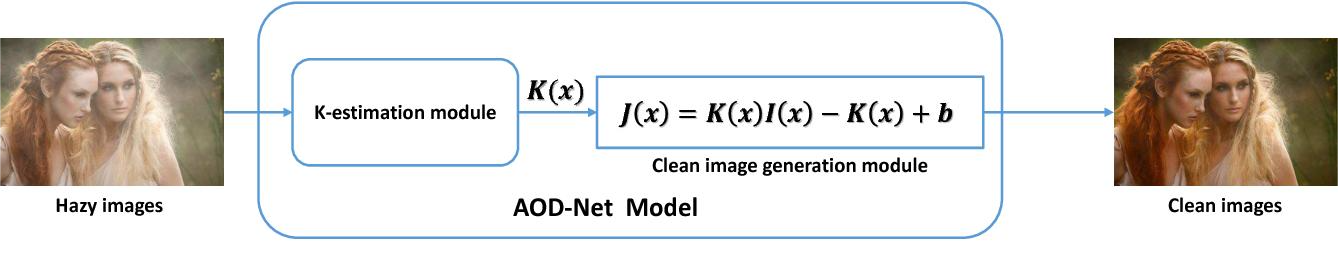
\includegraphics[width=\linewidth]{figures/pic11.png}
      \caption{AOD-Net结构示意图}
    \end{figure}
    \end{frame}

    \begin{frame}
      \frametitle{AOD-Net}
      \begin{figure}[h]
        \centering
        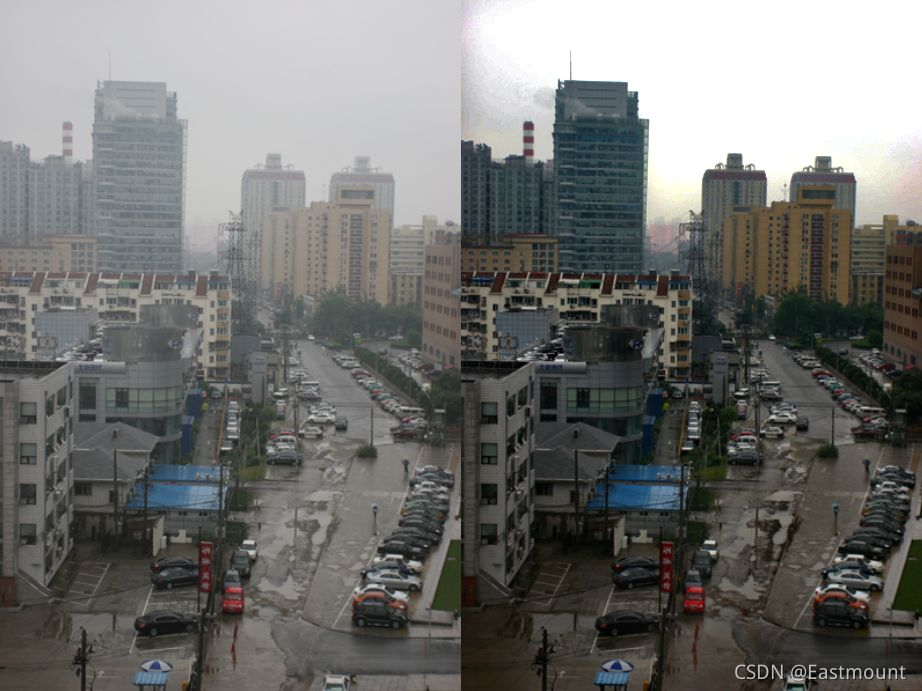
\includegraphics[width=0.8\linewidth]{figures/pic13.jpg}
        \caption{AOD-Net去雾效果图}
      \end{figure}
    \end{frame}

